\section{Impact of Excitation-Current Coordinate Reduction on Flux-Linkage Reconstruction Accuracy}\label{sec:mapreduction}
\subsection{Question and exact reduction condition}
The processing hypothesis is that a substantial discrepancy appears when the separate excitation measurements are projected, merged, rasterized, and queried as a single two-dimensional flux map. This section compares the actual saved artifacts with their own source measurements. A reconstruction discrepancy alone does not prove a physical dimensional-reduction error.

At fixed reduced coordinates \(s=i_d+ki_e\) and \(q=i_q\), the chain rule gives
\begin{equation}\label{eq:fiberresidual}
\left.\frac{\partial\widehat{\ps}}{\partial i_e}\right|_{s,q}
=\begin{bmatrix}L_{de}\\L_{qe}\end{bmatrix}
-k\begin{bmatrix}L_{dd}\\L_{qd}\end{bmatrix}
=\bvec-k\avec.
\end{equation}
Along any admissible connected constant-\((s,q)\) section,
\begin{equation}
\ps(s-ke_2,q,e_2)-\ps(s-ke_1,q,e_1)
=\int_{e_1}^{e_2}(\bvec-k\avec)(s-ke,q,e)\,\dd e.
\end{equation}
Thus the reduction preserves all stator-flux information under the conditions established in Section~\ref{sec:common}: both coupling equations must hold, together with the domain connectivity requirement. A violation at a point prevents an exact reduction in its neighborhood for that constant \(k\). The derivative estimates are numerical diagnostics of this condition, not exact measurements of its violation.

The pure coordinate shear leaves each source flux value unchanged. If two physical points have identical reduced coordinates but different fluxes, no single-valued reduced function can reproduce both. Here all projected measured coordinates are distinct: 7476 of 7476 in Set 1 and 8092 of 8092 in Set 2. Consequently, exact source-node interpolation is possible even for a physically unsuitable reduction. The triangulation may then represent incompatible slices through strong variations between nearby nodes.

\subsection{Saved representations and coordinate conventions}
The standalone script \texttt{analyze\_flux\_map\_reduction.m} loads the original local FluxEval files and evaluates:
\begin{itemize}
\item A: \texttt{Meas.PE\_psi\_d\_meas} and \texttt{PE\_psi\_q\_meas} at actual measured \((i_d,i_q,i_e)\).
\item B: \texttt{LUT.CtrlMaps.complete}, retaining separate source excitation-reference slices.
\item C: \texttt{LUT.CtrlMaps}, queried at measured \((i_d+ki_e,i_q)\), using its saved \texttt{EESM\_winding\_ratio}.
\end{itemize}
The saved factors are \(13.490937385\) for Set 1 and \(13.516845982\) for Set 2. Each slice is associated with its matching \texttt{complete.I\_exc\_vec} value, rather than an assumed field or array order.

The saved \texttt{complete} files have no coordinate metadata, and their d breakpoints coincide with the corresponding physical \texttt{Calc.Grid.Id\_fine} axes. The script queries them with measured physical \(i_d\). Newer local \texttt{Torque\_LUT\_Calc.m} source also supports relabelled complete slices with
\[
d_{\mathrm{slice}}^*=i_d+k_{\mathrm{slice}}I_{e,\mathrm{ref}}.
\]
For those slices, the documented \texttt{Coordinates.d\_axis} is used and the query receives the fixed slice-reference offset. Substituting pointwise measured \(i_e\) into that relabelling would change the physical lookup location within the already constructed slice. The merged map, in contrast, is built from pointwise measured excitation currents and requires those same measured currents at lookup.

Both B and C are queried with bilinear \texttt{interp2}. Out-of-domain or NaN-contaminated interpolation cells remain invalid; no extrapolation or zero filling is used. This specifies the diagnostic lookup operator, not the operator of every GUI or controller consumer. Nominal excitation values only assign groups. Requested stator currents are never substituted for measured query coordinates.

B is a collection of separate two-dimensional representations of the recorded groups, not a continuously interpolated three-current model. Small excitation-current fluctuations within each group remain present in its source data. Only the 3000 rpm group is available in the two selected full evaluations, so no comparison across machine speeds is possible here.

\subsection{Residuals, coverage, and saved-map comparison}
For \(x\in\{d,q\}\), define
\[
r_{x,B}=\psi_{x,B}-\psi_{x,A},\qquad r_{x,C}=\psi_{x,C}-\psi_{x,A}.
\]
A method's own mask requires both returned flux components to be finite. The common mask is the intersection of these masks. RMSE and maximum absolute residual are calculated componentwise on the stated mask. Figures comparing B with C use the common mask; the MAT output retains both masks, both summaries, and per-excitation summaries.

\begin{table}[htbp]
\centering\small
\caption{Saved-map reconstruction errors, all in mWb. Own support is method-specific; common support uses identical points for B and C within each dataset. Source counts are 7476 and 8092.}\label{tab:savedmaps}
\begin{tabular}{cllrrrrr}
\toprule
Set & Map & Mask & \(N\) & RMSE d & RMSE q & Max d & Max q\\
\midrule
1 & B: complete & Own & 6761 & 0.292 & 0.178 & 7.503 & 1.870\\
1 & C: merged & Own & 7357 & 5.336 & 4.169 & 38.497 & 28.765\\
1 & B: complete & Common & 6759 & 0.292 & 0.178 & 7.503 & 1.870\\
1 & C: merged & Common & 6759 & 5.538 & 4.331 & 38.497 & 28.765\\
\midrule
2 & B: complete & Own & 7319 & 0.313 & 0.177 & 7.392 & 1.792\\
2 & C: merged & Own & 7968 & 5.665 & 4.173 & 44.725 & 29.880\\
2 & B: complete & Common & 7315 & 0.313 & 0.174 & 7.392 & 1.751\\
2 & C: merged & Common & 7315 & 5.884 & 4.333 & 44.725 & 29.880\\
\bottomrule
\end{tabular}
\end{table}

The complete slices reproduce their source measurements much more closely on average than the merged map. Their maxima show that even B is not exact. Its residual includes the existing individual map construction and the bilinear return; the separate excitation maps have already been resampled.

Figures~\ref{fig:savedset1} and~\ref{fig:savedset2} show both components against source values, physical current-space residuals, and RMSE by excitation reference. In Set 2 the merged d-flux RMSE ranges from approximately \(3.85\) to \(8.12\) mWb across groups. The q-flux RMSE is approximately \(1.99\) mWb at 20 A and \(7.25\) mWb at 40 A. Set 1 shows a similar increase towards high excitation. Thus the discrepancy is structured in current space and excitation, rather than a single constant flux offset.

\begin{figure}[p]
\centering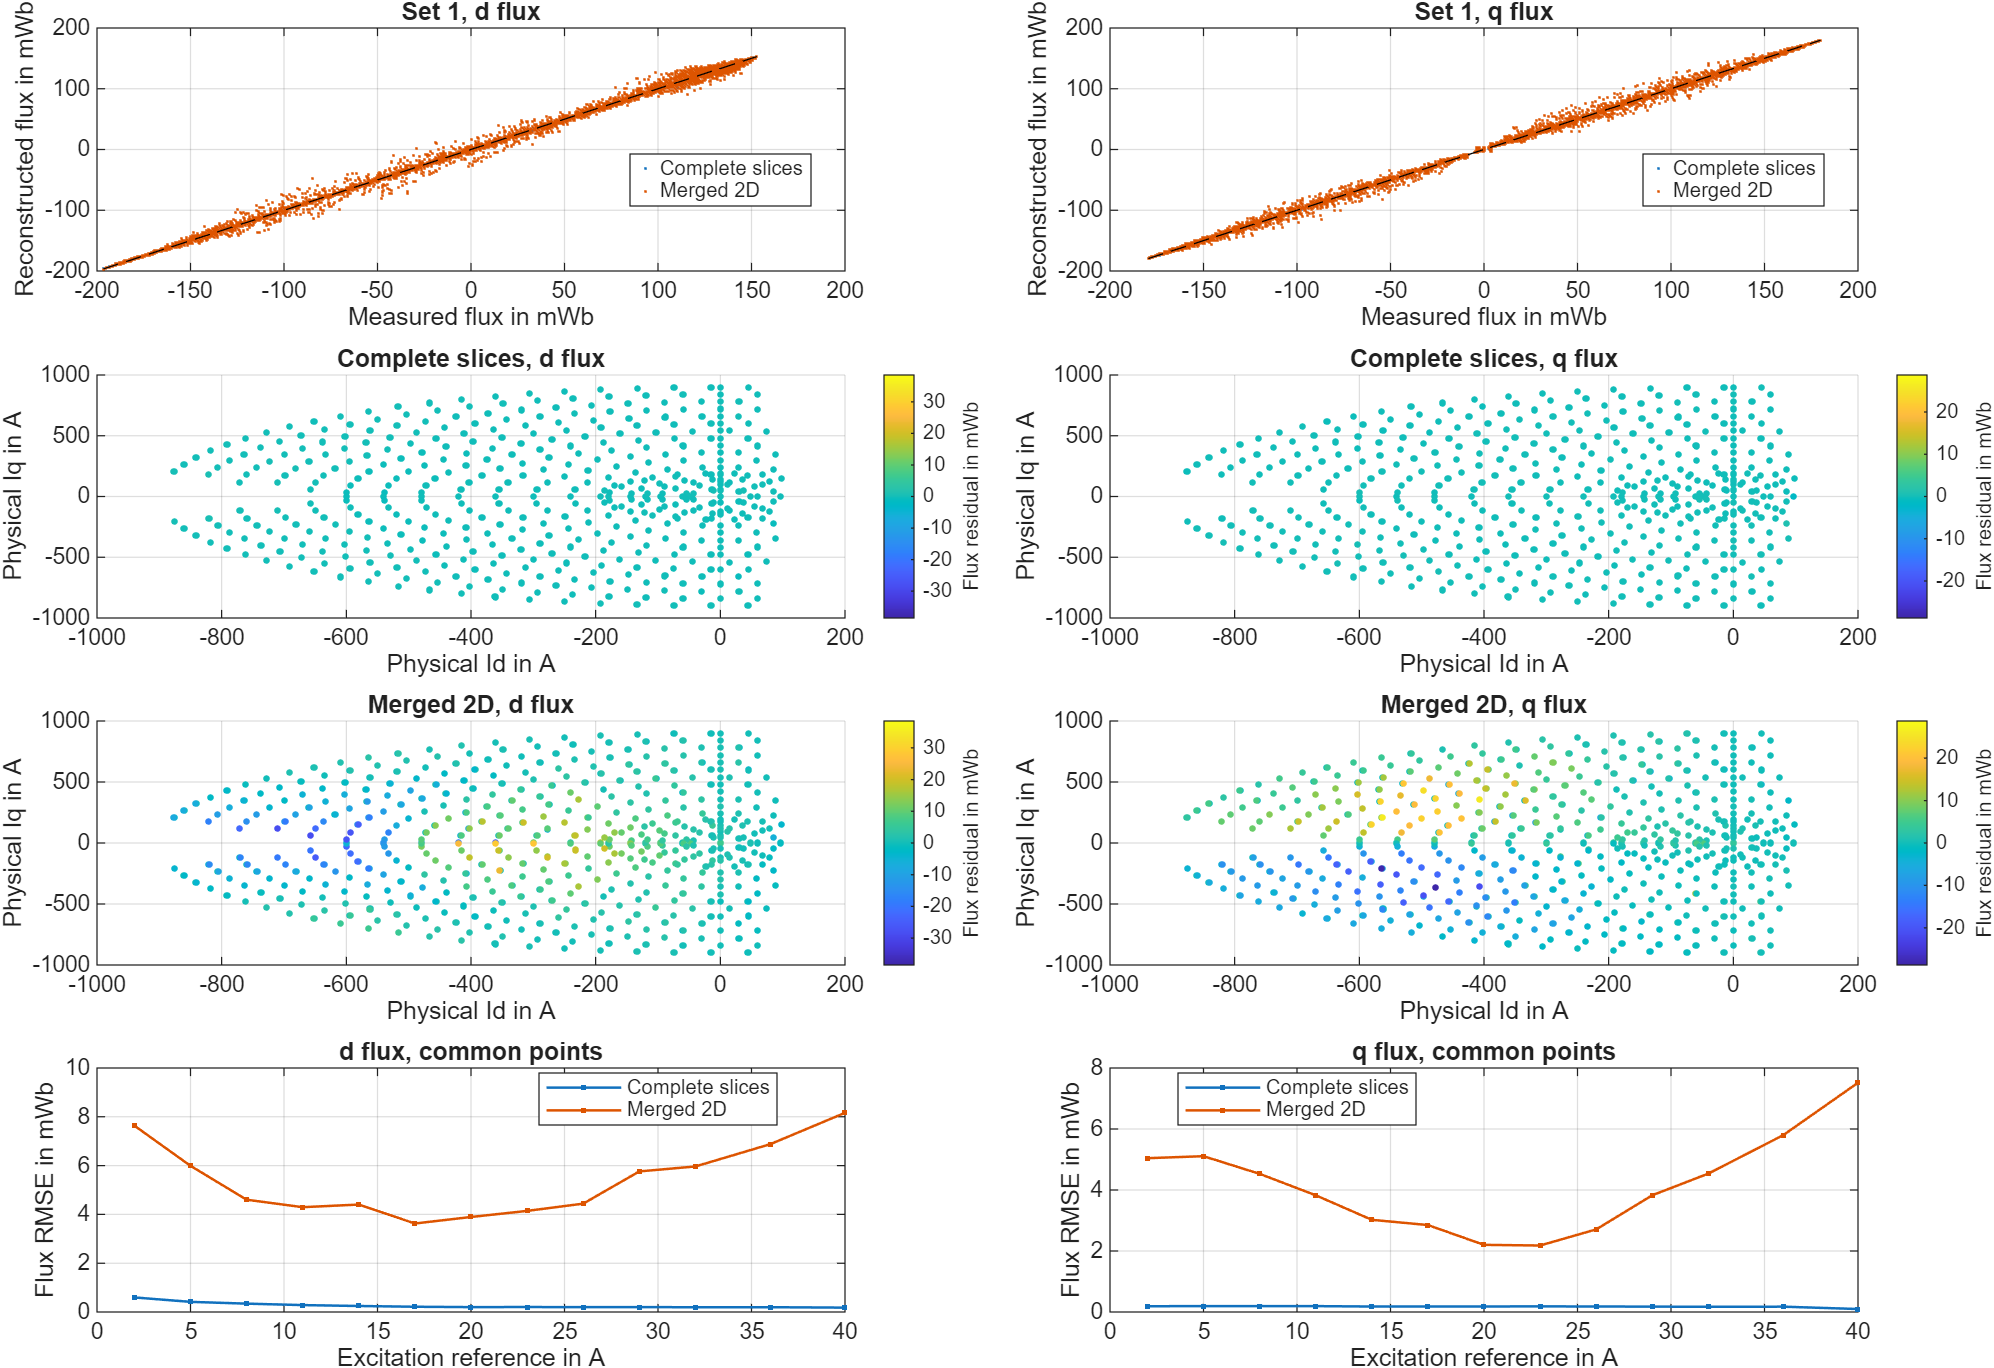
\includegraphics[width=\linewidth,height=0.84\textheight,keepaspectratio]{reduction_set1.png}
\caption{Set 1 on 6759 common points. Rows: reconstructed versus measured flux, complete-slice residuals, merged-map residuals, and per-group RMSE. Residuals are returned minus measured. Within each flux component the spatial panels share color limits. Spatial plots overlay excitation groups; bottom panels retain group distinctions.}\label{fig:savedset1}
\end{figure}
\begin{figure}[p]
\centering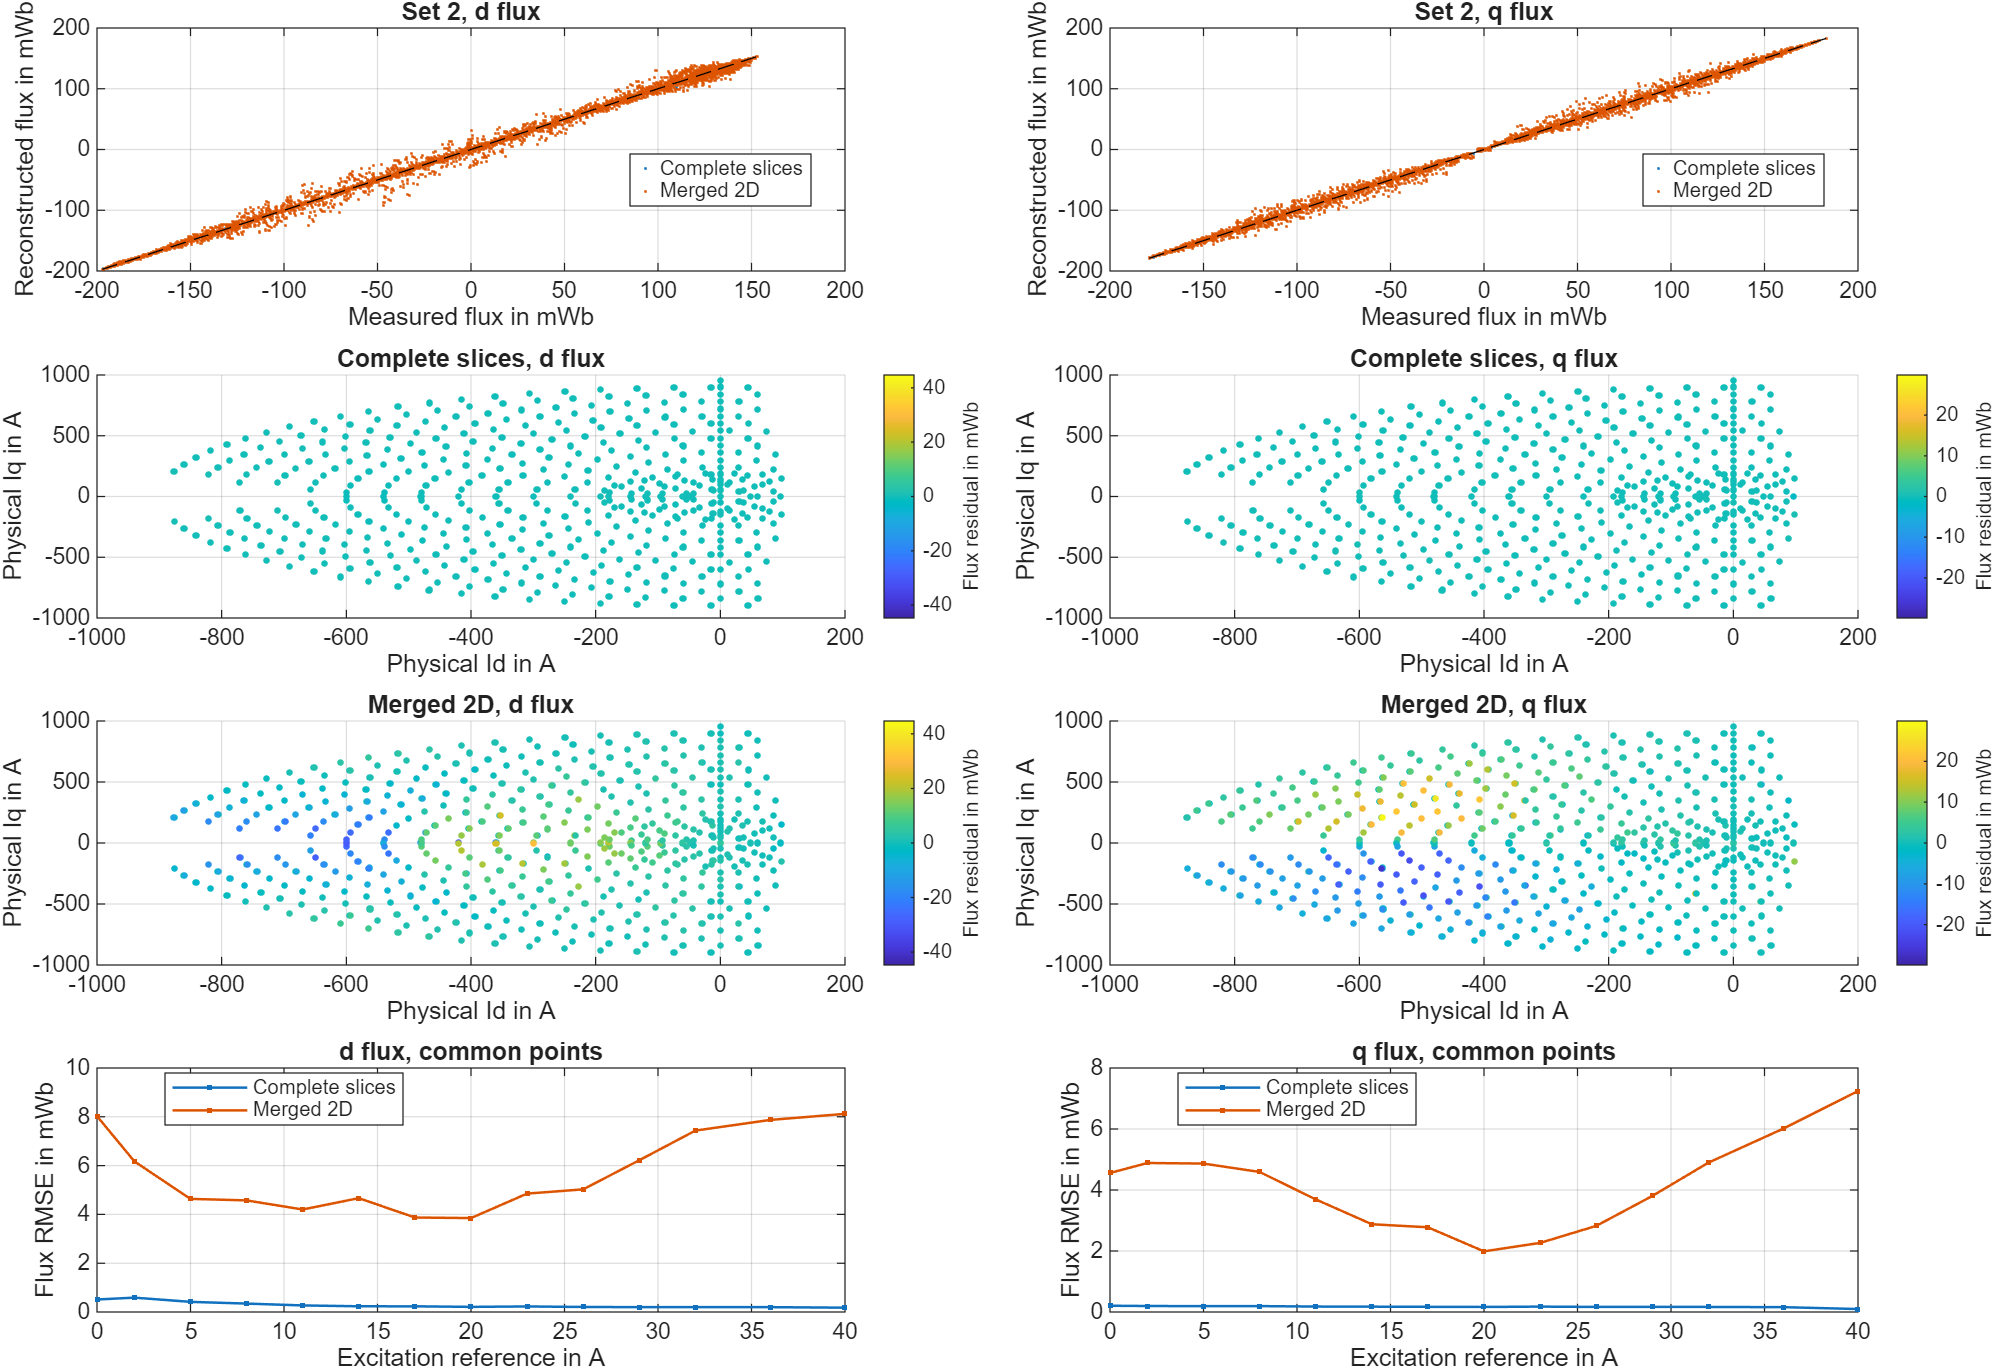
\includegraphics[width=\linewidth,height=0.84\textheight,keepaspectratio]{reduction_set2.png}
\caption{Set 2 on 7315 common points. Complete-slice residuals are close to zero on the color scale required for the merged residuals. Each group uses its own common-point subset: the bottom panels do not imply identical physical current support across excitation references.}\label{fig:savedset2}
\end{figure}

\subsection{Separating source arithmetic, gridding, and model reduction}
Using stored averaged measured voltages, measured stator currents, stored \(R_s\), and averaged electrical angular speed, the stationary formulas reproduce A to a maximum absolute discrepancy below \(1.4\,10^{-17}\) Wb. This establishes arithmetic consistency with the saved processed signals. It cannot establish their absolute calibration or rule out errors inherited from measurement and preprocessing.

The saved map branches are parallel. Complete slices originate in individual \texttt{Calc.Grid} representations, whereas the merged flux grid is constructed directly from sheared measured flux samples. B is not an intermediate stage through which C necessarily passes. Subtracting their RMSE values, or assigning the squared-error difference to one independent physical cause, would be unjustified.

Rebuilding the saved merged grid from measured projected points with linear scattered interpolation reproduces its finite flux values to roundoff. The scattered field also reproduces original source nodes to roundoff. The nonzero C--A residual therefore appears when that same scattered field is sampled onto the saved regular grid and bilinearly returned to source coordinates. This gives a direct operational explanation of the observed saved-map return error without requiring a new flux calculation or a changed machine speed.

To quantify this operation, keep the saved factor, saved axis extents, and underlying scattered field fixed, and vary only regular-grid size. These extents differ from the measured-coordinate bounds of the earlier controlled experiment in Section~\ref{sec:numerics}. Use one common finite mask across resolutions, restricted to original merged-map support.

\begin{table}[htbp]
\centering\small
\caption{Raster roundtrip on saved axis extents and fixed masks. Errors are in mWb. The 101-node row reproduces the saved map's own-support result.}\label{tab:savedraster}
\begin{tabular}{crrrrrr}
\toprule
Set & Nodes per axis & \(N\) & RMSE d & RMSE q & Max d & Max q\\
\midrule
1 & 101 & 7357 & 5.336 & 4.169 & 38.497 & 28.765\\
1 & 201 & 7357 & 3.991 & 2.809 & 39.696 & 29.679\\
1 & 401 & 7357 & 2.721 & 1.779 & 40.154 & 24.578\\
2 & 101 & 7968 & 5.665 & 4.173 & 44.725 & 29.880\\
2 & 201 & 7968 & 4.235 & 2.810 & 43.216 & 29.419\\
2 & 401 & 7968 & 2.977 & 1.742 & 42.143 & 23.468\\
\bottomrule
\end{tabular}
\end{table}

Average errors decrease substantially with resolution, but large maxima remain and need not decrease monotonically. This is consistent with steep local variations in the merged scattered field; it does not demonstrate that every such variation arises from invalid physical reduction. Exact source-node return is also not evidence of lossless reduction: interpolation has seen every source value. The missing-excitation-group experiment in Section~\ref{sec:holdout} supplies the complementary prediction check.

\subsection{A small constant-factor variation}
The script repeats the merged construction for \(k=12,12.5,\ldots,16\), additionally including each saved factor. Saved \(101\times101\) axis coordinates remain fixed. Each candidate changes projected measured points, triangulation, and query positions, while retaining source flux values. A single mask is used for every candidate and both components, also restricted to B--C common support: 6658 points in Set 1 and 7196 in Set 2.

The best sampled candidate minimizes \(\operatorname{RMSE}_d^2+\operatorname{RMSE}_q^2\). All measured samples also train these fields. This is a reconstruction diagnostic, not predictive factor selection; intermediate candidate values have not been optimized.

\begin{table}[htbp]
\centering\small
\caption{Saved and best sampled factors on fixed sweep masks. Errors are in mWb; \(k\) is in A/A. These masks differ from Table~\ref{tab:savedmaps}.}\label{tab:ksweep}
\begin{tabular}{clrrrrrr}
\toprule
Set & Candidate & \(k\) & \(N\) & RMSE d & RMSE q & Max d & Max q\\
\midrule
1 & Saved & 13.49094 & 6658 & 5.575 & 4.362 & 38.497 & 28.765\\
1 & Best sampled & 14.00000 & 6658 & 4.879 & 4.120 & 32.135 & 28.142\\
2 & Saved & 13.51685 & 7196 & 5.928 & 4.368 & 44.725 & 29.880\\
2 & Best sampled & 14.50000 & 7196 & 5.067 & 4.043 & 31.094 & 25.916\\
\bottomrule
\end{tabular}
\end{table}

The combined RMS magnitude decreases by approximately 9.8 percent in Set 1 and 12.0 percent in Set 2. Neither candidate approaches the average accuracy of the separate saved slices. The d and q components prefer different trends as \(k\) changes, consistent with satisfying two flux constraints together. The best sampled reconstruction factor need not equal the derivative-based global factor: objectives and interpolation effects differ.

\begin{figure}[htbp]
\centering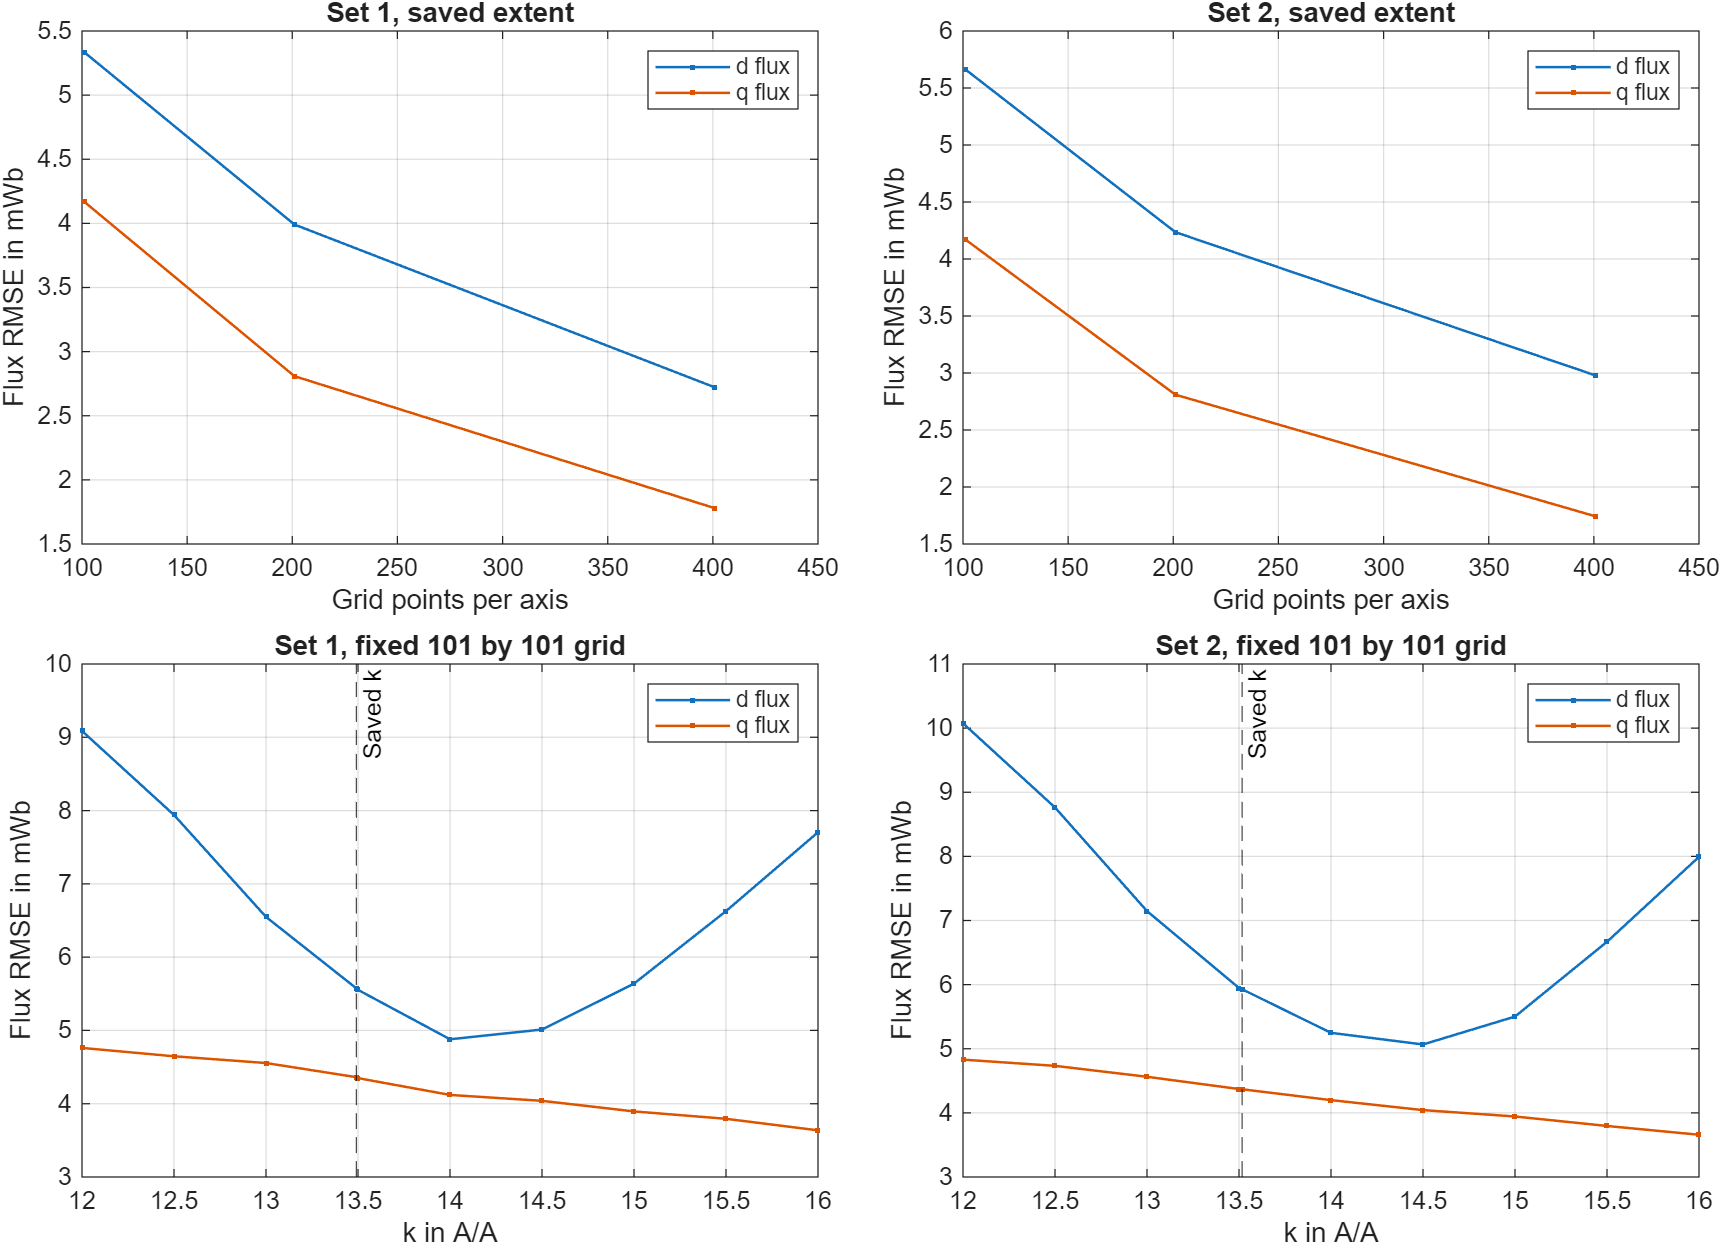
\includegraphics[width=\linewidth]{reduction_processing.png}
\caption{Saved-extent raster refinement at fixed saved \(k\) (top) and the small \(k\) sweep at fixed raster axes (bottom). Masks are fixed within each comparison but differ between top and bottom. Dashed lines mark saved factors.}\label{fig:reductionprocessing}
\end{figure}

\subsection{Established findings and consequence for MeasEval}
\begin{enumerate}
\item The coordinate shift itself changes no flux value. The stationary calculation is consistent with stored inputs to roundoff; absolute measurement accuracy remains unresolved.
\item Individual slice construction and lookup introduce small average residuals, with some larger isolated errors.
\item The actual merged-grid roundtrip creates much larger reconstruction residuals. Refinement demonstrably reduces their average magnitude. This identifies an interpolation and representation effect at the original measurement speed.
\item Changing one constant factor improves the tested result moderately but does not remove its discrepancy. This sweep cannot assign a numerical percentage to physical information loss: it also changes triangulation and raster sampling.
\item The separate derivative and whole-group holdout results provide additional evidence against an exact common constant reduction over this domain. The tested three-current predictor has lower missing-group errors. A complete causal partition of measurement noise, interpolation, and structural reduction error is not identified.
\end{enumerate}
A full three-current representation retains excitation explicitly and avoids imposing equation~\eqref{eq:fiberresidual} as zero. It still needs adequate sampling, suitable interpolation, and reliable measurements; it is not automatically exact. The evidence favors investigating it when accuracy across excitation is required. Improving the constant factor and raster resolution remain useful approximations, but their benefit should be checked with withheld excitation groups rather than source-node reconstruction alone.

